\documentclass[tikz, border=3mm]{standalone}

\usepackage{amsmath}
\usepackage{amssymb}
\usepackage{mathtools}
\usepackage[dvipsnames]{xcolor}
\usetikzlibrary{positioning, arrows.meta, fit, backgrounds, shapes.geometric, calc}

\begin{document}

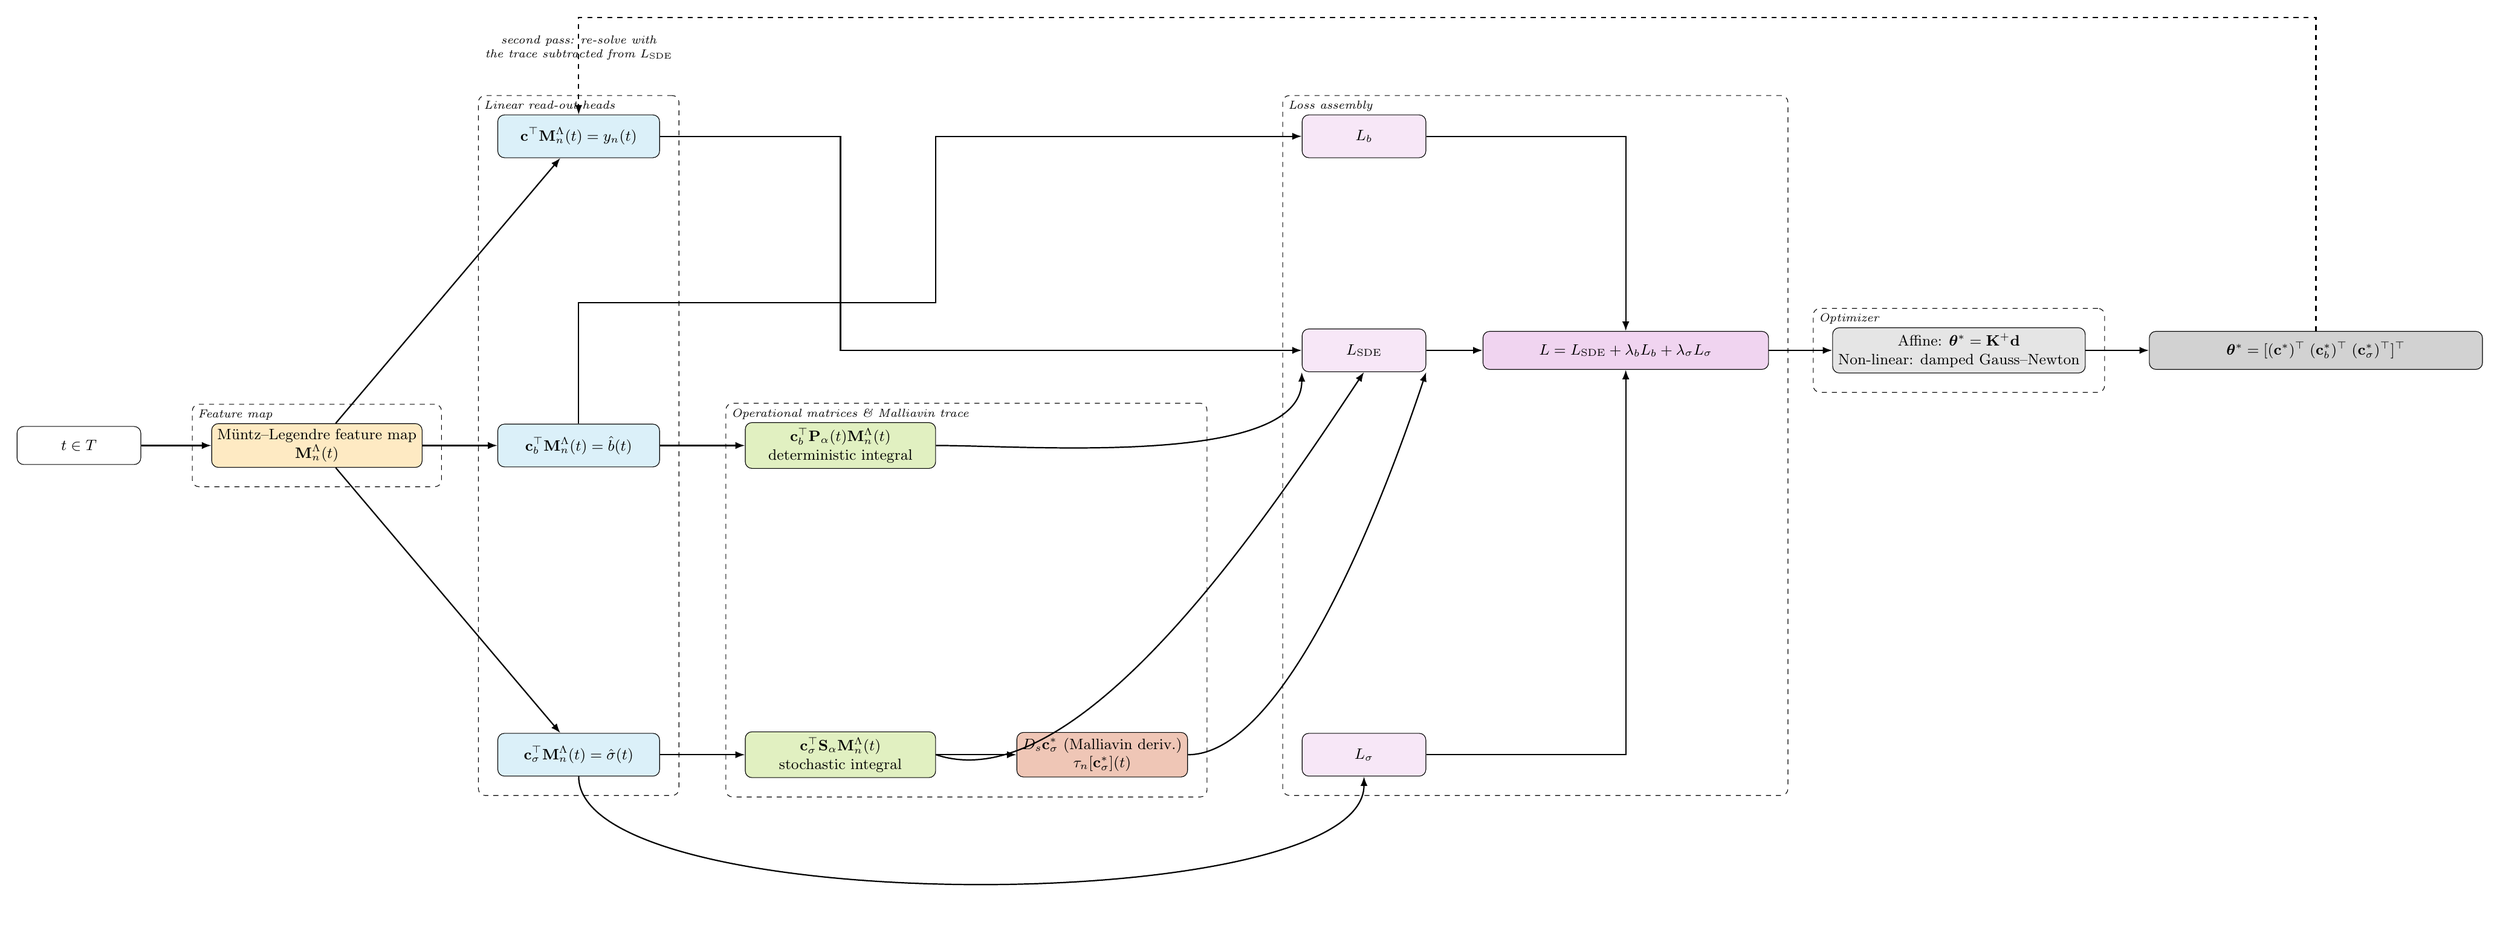
\begin{tikzpicture}[
    every node/.style = {font = \small},
    io/.style        = {draw, rounded corners, fill = white, minimum height = 8mm, minimum width = 26mm, align = center},
    layer/.style      = {draw, rounded corners, fill = Dandelion!25, minimum height = 9mm, minimum width = 40mm, align = center},
    head/.style       = {draw, rounded corners, fill = SkyBlue!30, minimum height = 9mm, minimum width = 34mm, align = center},
    opmat/.style      = {draw, rounded corners, fill = YellowGreen!30, minimum height = 9mm, minimum width = 40mm, align = center},
    trace/.style      = {draw, rounded corners, fill = BrickRed!20, minimum height = 9mm, minimum width = 34mm, align = center},
    loss/.style       = {draw, rounded corners, fill = Plum!25, minimum height = 9mm, minimum width = 26mm, align = center},
    opt/.style        = {draw, rounded corners, fill = Gray!20, minimum height = 9mm, minimum width = 50mm, align = center},
    arr/.style        = {-{Latex[length=2mm]}, thick},
    darr/.style       = {-{Latex[length=2mm]}, thick, dashed},
    grouplabel/.style = {font = \scriptsize\itshape, anchor = north west},
]

% ---------- explicit grid: (x, y) in cm, left to right pipeline ----------
\node[io]    (t)         at ( 0.0,  0.0) {$t \in T$};
\node[layer] (basis)     at ( 5.0,  0.0) {M\"untz--Legendre feature map \\ $\mathbf M_n^\Lambda(t)$};

\node[head]  (chead)     at (10.5,  6.5) {$\mathbf c^\top \mathbf M_n^\Lambda(t) = y_n(t)$};
\node[head]  (bhead)     at (10.5,  0.0) {$\mathbf c_b^\top \mathbf M_n^\Lambda(t) = \hat b(t)$};
\node[head]  (shead)     at (10.5, -6.5) {$\mathbf c_\sigma^\top \mathbf M_n^\Lambda(t) = \hat \sigma(t)$};

\node[opmat] (Pop)       at (16.0,  0.0) {$\mathbf c_b^\top \mathbf P_\alpha(t)\mathbf M_n^\Lambda(t)$ \\ deterministic integral};
\node[opmat] (Sop)       at (16.0, -6.5) {$\mathbf c_\sigma^\top \mathbf S_\alpha \mathbf M_n^\Lambda(t)$ \\ stochastic integral};

\node[trace] (trace)     at (21.5, -6.5) {$D_s\mathbf c_\sigma^*$ (Malliavin deriv.) \\ $\tau_n[\mathbf c_\sigma^*](t)$};

\node[loss]  (Lb)        at (27.0,  6.5) {$L_b$};
\node[loss]  (Lsde)      at (27.0,  2.0) {$L_{\mathrm{SDE}}$};
\node[loss]  (Ls)        at (27.0, -6.5) {$L_\sigma$};

\node[io, fill=Plum!45, minimum width=60mm] (L) at (32.5, 2.0) {$L = L_{\mathrm{SDE}} + \lambda_bL_b + \lambda_\sigma L_\sigma$};

\node[opt]   (opt)       at (39.5, 2.0) {Affine: $\boldsymbol \theta^* = \mathbf K^+\mathbf d$ \\ Non-linear: damped Gauss--Newton};

\node[io, fill=Gray!35, minimum width=70mm] (thetastar) at (47.0, 2.0) {$\boldsymbol \theta^* = [(\mathbf c^*)^\top \; (\mathbf c_b^*)^\top \; (\mathbf c_\sigma^*)^\top]^\top$};

% ---------- forward pass (first, uncorrected pass) ----------
\draw[arr] (t) -- (basis);
\draw[arr] (basis) -- (chead);
\draw[arr] (basis) -- (bhead);
\draw[arr] (basis) -- (shead);

\draw[arr] (bhead) -- (Pop);
\draw[arr] (shead) -- (Sop);
\draw[arr] (Sop) -- (trace);
\draw[arr] (shead.south) .. controls +(0,-3) and +(0,-3) .. (Ls.south);

\draw[arr] (bhead.north) -- (10.5,3) -- (18,3) -- (18,6.5) -- (Lb.west);
\draw[arr] (chead.east) -- (16,6.5) -- (16,2) -- (Lsde.west);
\draw[arr] (Pop.east) .. controls +(2,0) and +(0,-2) .. (Lsde.south west);
\draw[arr] (Sop.east) .. controls +(3,-1) and +(-2,-3) .. (Lsde.south);
\draw[arr] (trace.east) .. controls +(2,0) and +(-1,-3) .. (Lsde.south east);

\draw[arr] (Lb.east) -| (L.north);
\draw[arr] (Lsde.east) -- (L.west);
\draw[arr] (Ls.east) -| (L.south);

\draw[arr] (L) -- (opt);
\draw[arr] (opt) -- (thetastar);

% ---------- second, trace-corrected pass (computed once, not iterated) ----------
\draw[darr] (thetastar.north) -- (47.0,9) -- (10.5,9) -- (chead.north)
    node[midway, above, align=center, font=\scriptsize\itshape] {second pass: re-solve with\\the trace subtracted from $L_{\mathrm{SDE}}$};

% ---------- background grouping ----------
\begin{scope}[on background layer]
    \node[draw, dashed, rounded corners, inner sep=4mm, fit=(basis)] (g1) {};
    \node[grouplabel] at (g1.north west) {Feature map};

    \node[draw, dashed, rounded corners, inner sep=4mm, fit=(chead)(bhead)(shead)] (g2) {};
    \node[grouplabel] at (g2.north west) {Linear read-out heads};

    \node[draw, dashed, rounded corners, inner sep=4mm, fit=(Pop)(Sop)(trace)] (g3) {};
    \node[grouplabel] at (g3.north west) {Operational matrices \& Malliavin trace};

    \node[draw, dashed, rounded corners, inner sep=4mm, fit=(Lb)(Lsde)(Ls)(L)] (g4) {};
    \node[grouplabel] at (g4.north west) {Loss assembly};

    \node[draw, dashed, rounded corners, inner sep=4mm, fit=(opt)] (g5) {};
    \node[grouplabel] at (g5.north west) {Optimizer};
\end{scope}

\end{tikzpicture}

\end{document}
